\documentclass[10pt]{article}
\usepackage[letterpaper,top=0.55in,bottom=0.58in,left=0.62in,right=0.62in]{geometry}
\usepackage[T1]{fontenc}
\usepackage[utf8]{inputenc}
\usepackage{lmodern}
\usepackage{microtype}
\usepackage{graphicx}
\usepackage{booktabs}
\usepackage{array}
\usepackage{enumitem}
\usepackage{titlesec}
\usepackage{xcolor}
\usepackage{tikz}
\usetikzlibrary{arrows.meta,positioning,shapes.geometric,fit}
\usepackage{amsmath,amssymb}
\usepackage{hyperref}
\usepackage{multicol}
\usepackage{caption}

\definecolor{ink}{HTML}{17243A}
\definecolor{blue}{HTML}{1B5EA7}
\definecolor{cyan}{HTML}{DCEFF6}
\definecolor{gold}{HTML}{C58B1B}
\definecolor{soft}{HTML}{F3F5F7}
\hypersetup{colorlinks=true,linkcolor=blue,urlcolor=blue,citecolor=blue}
\color{ink}
\setlength{\parindent}{0pt}
\setlength{\parskip}{2pt}
\setlength{\columnsep}{14pt}
\setlist[itemize]{leftmargin=1.3em,itemsep=0pt,topsep=2pt,parsep=0pt}
\setlist[enumerate]{leftmargin=1.5em,itemsep=0pt,topsep=2pt,parsep=0pt}
\titleformat{\section}{\large\bfseries\color{blue}}{}{0pt}{}[\vspace{-2pt}\color{cyan}\titlerule]
\titleformat{\subsection}{\normalsize\bfseries\color{ink}}{}{0pt}{}
\titlespacing*{\section}{0pt}{4pt}{2pt}
\titlespacing*{\subsection}{0pt}{4pt}{1pt}
\captionsetup{font=footnotesize,labelfont=bf,skip=2pt}
\pagestyle{plain}

\newcommand{\armT}{\textsc{Time}}
\newcommand{\armC}{\textsc{Cost}}
\newcommand{\armB}{\textsc{Baseline}}
\newcommand{\E}{\mathbb{E}}

\begin{document}

\begin{center}
{\LARGE\bfseries Faces or Facts?}\par
\vspace{1pt}
{\large Experimental Evidence on Time Pressure, Information Costs, and Gender Bias in Electoral Choice}\par
\vspace{3pt}
{\normalsize Nayssa Alejandra Mar\'in D\'iaz \quad Andrea Canales \quad H\'ector Bahamonde}\par
\vspace{1pt}
{\small Design and analysis proposal --- work in progress --- 1 October 2026}
\end{center}

\vspace{-3pt}
\noindent\colorbox{cyan}{\parbox{0.978\linewidth}{\small
\textbf{Abstract.} Voters often see a candidate's face before they read a platform. Building on evidence that rapid visual impressions can predict election winners, we ask when time pressure and information costs displace political learning, and whether that displacement exposes women candidates to distinctive scrutiny. We field a three-arm online visual conjoint experiment using photographs and programmatic information from Colombian electoral data. Eligible adults outside Colombia complete five practice and fifteen consequential paired-profile choices. Respondents are assigned to a 10-second deadline, a cognitive cost for revealing political information, or an unconstrained baseline. Candidate pairs and left-right positions are randomized within respondents. We record vote choice, candidate-specific information reveals, response time, treatment exposure, and the complete candidate-source row shown in every task. The design identifies intention-to-treat effects of decision environments and causal effects of assigning complete candidate profiles. Because the attributes within a real candidate profile are not independently randomized, gender-, ideology-, and appearance-based contrasts describe bundled profiles rather than conventional attribute-level AMCEs.}}

\section{Faces arrive before facts}

Most political choices begin with a sequence so ordinary that it is easy to overlook: voters see a face before they read a platform. A visual impression arrives almost automatically, whereas learning a candidate's ideology and priorities requires time and effort. This ordering matters because judgments made from faces can form after exposures as brief as 100 milliseconds and predict real election outcomes (Todorov et al. 2005). The familiar contrast between ``faces'' and ``facts'' is therefore not merely rhetorical. It describes two sources of political judgment that become available at different speeds and costs.

The relevant cognitive framework is dual processing, but not the claim that a stopwatch cleanly turns ``System 1'' on and ``System 2'' off. Type 1 processes are rapid and autonomous; Type 2 processes support hypothetical comparison and draw heavily on working memory (Evans and Stanovich 2013). Under time pressure, people adapt by accelerating processing, filtering cues, or substituting a simpler noncompensatory rule for effortful integration (Payne, Bettman, and Luce 1996; Rieskamp and Hoffrage 2008). Political learning follows the same basic logic. Candidate evaluations can be updated on-line as information is encountered, even when the facts supporting the resulting impression are poorly remembered (Lodge, McGraw, and Stroh 1989). A deadline therefore changes which evidence can enter the running evaluation; it does not directly reveal an otherwise unobservable cognitive ``system.''

Antonakis and Dalgas (2009) make this puzzle unusually concrete. After an imaginary voyage from Troy to Ithaca, Swiss children aged 5--13 were shown pairs of photographs from French parliamentary runoffs and asked whom they would choose as captain. Their choices predicted the actual winner with a probability of 0.71; adults' competence ratings predicted the winner with a probability of 0.72, and the child and adult response patterns were statistically indistinguishable. The participants did not need campaign knowledge, policy positions, or electoral experience to reproduce the electorate's ranking. As Antonakis and Dalgas put it, ``voters are anchored in first impressions and do not appropriately correct initial inferences'' (2009, 1183). Ballew and Todorov (2007) identify the speed of this process more directly: competence judgments after 100 or 250 milliseconds were as predictive as judgments made with unlimited exposure, and a two-second response deadline preserved predictive accuracy while instructions to deliberate lengthened response time and reduced it.

That finding is compelling, but it leaves the central decision process unobserved. We know that faces can predict choices; we know much less about when voters stop at the face, when they seek political information, and whether constraints make one source dominate the other. Candidate photographs operate as cues in low-information elections (Banducci et al. 2008), appearance predicts success across political contexts (Rosar et al. 2008; Berggren et al. 2010; Lawson et al. 2010), and media exposure can strengthen appearance-based voting among less informed citizens (Lenz and Lawson 2011). Faces also convey perceived competence, ideology, party, status, and threat rather than attractiveness alone (Mattes et al. 2010; Herrmann and Shikano 2016; Olivola et al. 2018).

\subsection{Gendered scrutiny and the cost of learning}

Candidate gender can shape not only the final vote but the path by which voters learn. Ditonto, Hamilton, and Redlawsk (2014) show that voters seek more competence-related and ``compassion issue'' information about women than men. Andersen and Ditonto (2020) further show that the amount of search triggered by a woman candidate depends on partisan alignment and is strongest early in a campaign. This is consequential because women are often required to provide stronger evidence of qualification: across survey experiments, voters applied more stringent qualification standards to women candidates (Bauer 2020). A photograph makes candidate gender immediately available before policy text is opened, exactly the sequence in which an early cue can organize subsequent search.

The mechanism need not involve conscious hostility. Campaign communication can activate gender stereotypes that otherwise remain dormant (Bauer 2015), and rapid appearance-based inferences predict different outcomes by candidate gender: competence is most predictive in men-only races, whereas attractiveness predicts women-only races (Ditonto and Mattes 2018). Bahamonde and Sarpila (2024) likewise find a compounded penalty for working-class-looking women and weaker electoral returns to attractiveness for women than men. Recent work cautions against a universal penalty: eye-tracking evidence finds similar attention to stereotype-consistent and inconsistent information across candidate gender, suggesting that bias can arise from the standards applied to evidence rather than from attention alone (Jenke 2025), while think-aloud evidence shows both rapid gender heuristics and later gendered rationalizations (Rohrbach and Sch\"onhagen 2025). The empirical question is therefore not simply whether women lose. It is whether women profiles invite different information acquisition, whether constraints suppress potentially corrective learning, and whether the same evidence is translated into choice differently for women and men.

Our experiment turns these predictive and gendered puzzles into a causal process test. Every respondent sees the same visual choice, but we randomize whether decisions occur under a 10-second deadline, whether political information carries an effort cost, or whether neither constraint applies. We observe not only whom respondents choose, but whether they request ideological and programmatic information for each woman or man profile before choosing. The contribution is to locate inequality in the sequence from first impression, to information acquisition, to choice. Methodologically, the study combines temporal scarcity and information cost with click-level process measurement and repeated choices between profiles assembled from Colombian electoral data. Standard conjoint AMCEs require independently randomized attribute levels (Hainmueller, Hopkins, and Yamamoto 2014); because photograph, gender, ideology, electoral history, and facial measurements travel together here, primary causal claims concern the randomized decision environment and assigned \emph{whole profiles}, while component-feature analyses remain secondary.

\section{Design and implementation}

\textbf{Population and screening.} The planned sample is 462 adults aged 18--65, balanced across men and women and allocated approximately equally across the three arms ($154$ per arm). To minimize recognition and prior Colombian political knowledge, respondents must neither be Colombian nationals nor currently reside in Colombia, and must report never having lived in Colombia. Residence, nationality, and prior residence are asked sequentially so that an ineligible person exits immediately. Age, gender identity, occupation, education, turnout, political interest, discussion frequency, and left-right self-placement are then collected on one page.

\textbf{Stimuli and repeated choice.} The deployed candidate pool contains 71 profiles with nonmissing programmatic text in \texttt{base\_final\_merged.csv}. Each respondent receives 40 distinct profile assignments---two per round---randomized without replacement into five practice and fifteen analysis rounds. Within each round, the pair and left-right placement are randomized. A profile shows the candidate photograph and a button that can reveal the Spanish \texttt{Texto} field (ideology plus policy priorities). The binary outcome is the selected candidate. Fifteen main tasks are defensible in light of experimental evidence that substantially larger conjoint batteries produce only limited average satisficing in comparable online settings (Bansak et al. 2018); practice rounds are excluded from confirmatory estimates.

\begin{figure}[h!]
\centering
\begin{minipage}[t]{0.475\linewidth}
\centering
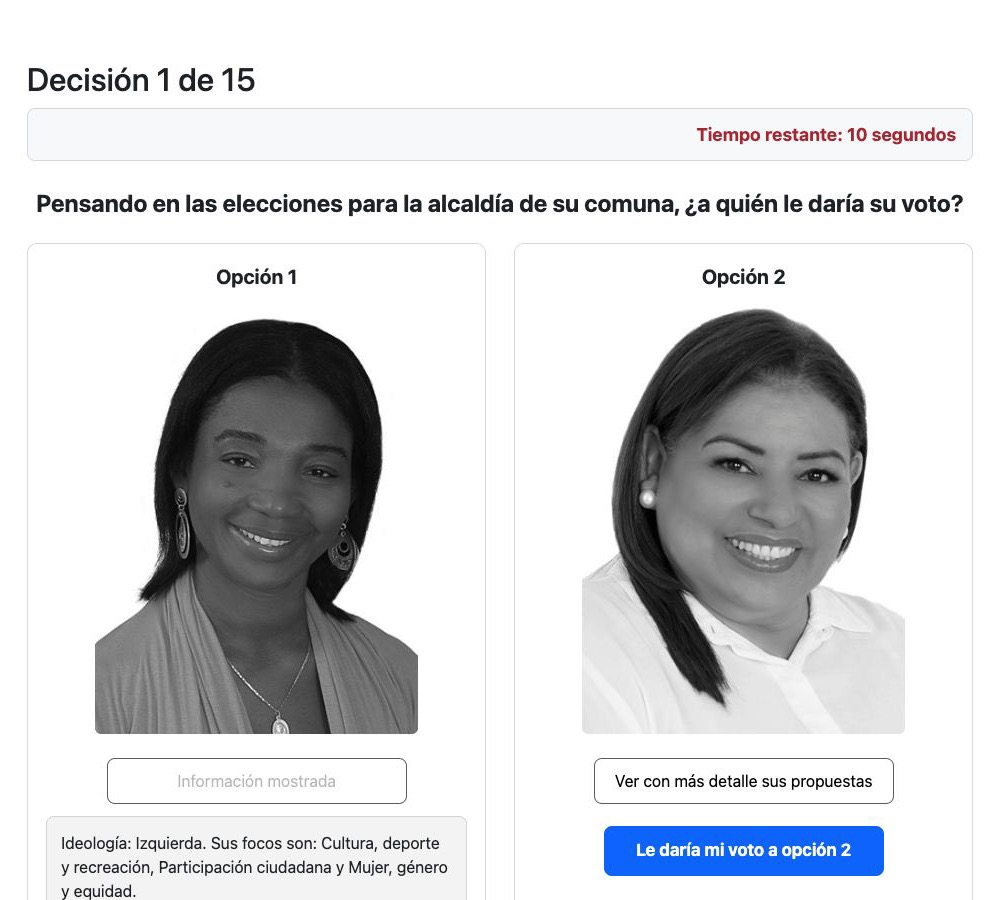
\includegraphics[width=\linewidth,height=1.88in,keepaspectratio]{visual_conjoint_task_example.jpg}
\caption*{\textbf{A. Task interface.} A live oTree task using Colombian candidate photographs; the left profile's programmatic text has been revealed.}
\end{minipage}\hfill
\begin{minipage}[t]{0.50\linewidth}
\centering
\resizebox{\linewidth}{!}{%
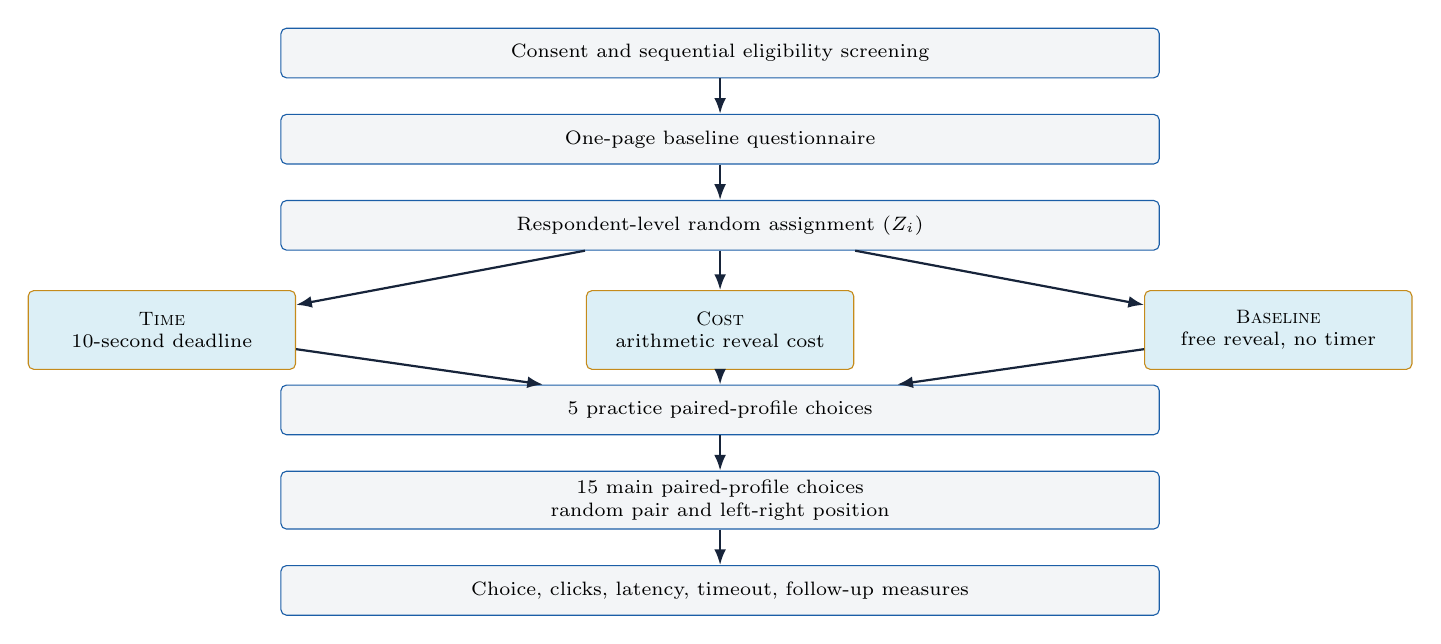
\begin{tikzpicture}[
  node distance=4.5mm and 5mm,
  box/.style={rounded corners=2pt,draw=blue,fill=soft,minimum width=0.92\linewidth,minimum height=6.3mm,align=center,font=\scriptsize},
  arm/.style={rounded corners=2pt,draw=gold,fill=cyan,minimum width=0.28\linewidth,minimum height=10mm,align=center,font=\scriptsize},
  arr/.style={-{Latex[length=2mm]},thick,draw=ink}
]
\node[box] (screen) {Consent and sequential eligibility screening};
\node[box,below=of screen] (survey) {One-page baseline questionnaire};
\node[box,below=of survey] (rand) {Respondent-level random assignment ($Z_i$)};
\node[arm,below left=5mm and -2mm of rand] (time) {\armT\\10-second deadline};
\node[arm,below=5mm of rand] (cost) {\armC\\arithmetic reveal cost};
\node[arm,below right=5mm and -2mm of rand] (base) {\armB\\free reveal, no timer};
\node[box,below=17mm of rand] (practice) {5 practice paired-profile choices};
\node[box,below=of practice] (main) {15 main paired-profile choices\\random pair and left-right position};
\node[box,below=of main] (follow) {Choice, clicks, latency, timeout, follow-up measures};
\draw[arr] (screen)--(survey);
\draw[arr] (survey)--(rand);
\draw[arr] (rand)--(time);
\draw[arr] (rand)--(cost);
\draw[arr] (rand)--(base);
\draw[arr] (time)--(practice);
\draw[arr] (cost)--(practice);
\draw[arr] (base)--(practice);
\draw[arr] (practice)--(main);
\draw[arr] (main)--(follow);
\end{tikzpicture}%
}
\caption*{\textbf{B. Assignment and measurement.} Treatment is fixed by respondent; profile pairing and side are rerandomized by round.}
\end{minipage}
\vspace{-6pt}
\end{figure}

\textbf{Experimental arms.} Let $Z_i\in\{T,C,B\}$ denote assignment. In \armT, each task has a visible 10-second countdown; information can otherwise be revealed freely. In \armC, there is no task deadline, but revealing a profile's text requires solving a simple arithmetic challenge. In \armB, there is neither a timer nor an arithmetic barrier, and the same text is available through the reveal button. The interface, candidate pool, task count, and choice prompt are otherwise held constant. The current design randomizes arms with equal probability at the respondent level.

\pagebreak
\textbf{What the ten-second deadline manipulates.} The cutoff is a theory-guided operational choice, not a universal boundary between intuition and deliberation. Political-face studies show that election-predictive impressions are already available after 100--250 milliseconds and remain predictive under a two-second response deadline (Ballew and Todorov 2007). At the other end of the decision, a voting experiment found mean response times of 16.63 seconds without opportunity time costs and 5.67 seconds when every additional second was costly; the latter condition also reduced deliberative strategic voting (Al\'os-Ferrer and Garagnani 2022). Those tasks are not numerically interchangeable with ours, but together they establish a useful range: faces can supply a choice-relevant cue almost immediately, whereas politically informed comparison occupies a longer interval. More generally, time pressure produces selective search, cue-wise processing, and lexicographic rather than fully compensatory integration (Payne, Bettman, and Luce 1996; Rieskamp and Hoffrage 2008). Our treatment therefore manipulates \emph{temporal scarcity in evidence acquisition}; it does not directly assign or measure ``System 1.''

\textbf{Why ten rather than two or approximately seventeen seconds.} The value is also tied to the geometry of the implemented task. Across the 71 usable Colombian candidate profiles, each Spanish description contains 10--17 words (median 14). Reading both median-length texts requires processing 28 words, in addition to inspecting two photographs, making two reveal decisions, comparing the information, and registering a vote. Meta-analytic adult silent-reading benchmarks are roughly 238 words per minute for English nonfiction and about 278 words per minute across the available Spanish studies (Brysbaert 2019). At those rates, reading 28 words alone takes approximately 6.0--7.1 seconds; the clicks, visual orientation, comparison, and choice consume additional time. This calculation is a descriptive benchmark, not an assumption that every respondent reads at the same speed. A two-second limit would make information acquisition nearly impossible and collapse the treatment toward a face-only task. A limit near the 16.63-second unconstrained voting mean would leave substantially more room for exhaustive search. Ten seconds is deliberately intermediate: it preserves a genuine opportunity to reveal and use at least one description, while making the revelation and integration of both descriptions costly.

\textbf{Pilot validation and decision rule.} The exact cutoff will be validated in a discarded pilot before outcome analysis. We will compare the timer and baseline arms on median decision time, the probability of revealing any text, the probability of revealing both texts, and timeout. The cutoff will be retained only if it (i) shortens decisions, (ii) reduces exhaustive two-profile revelation, (iii) leaves nondegenerate variation in whether at least one profile is revealed, and (iv) does not generate an excessive timeout rate. Operational thresholds for these four criteria will be written before inspecting the pilot. If ten seconds fails them, the interface will be recalibrated in the discarded pilot, and the final value will be frozen in the preregistration before production data are collected. The confirmatory estimand is therefore the intention-to-treat effect of the pre-specified ten-second environment, not the effect of an unobserved cognitive state.

\textbf{Recorded data and reproducibility.} Each task row stores arm, round, side assignment, displayed and chosen IDs, latency, timer status, candidate-specific reveals, total clicks, and follow-up responses. It also stores each candidate's complete 41-column source record---including gender, age, party, political text, geography, votes, and facial measures---as explicit left/right variables and a lossless JSON snapshot. Every choice remains reconstructable if the source file changes.

\section{Potential outcomes, estimands, and hypotheses}

For respondent $i$ in main task $t$, let $P_{it}=(C^L_{it},C^R_{it})$ denote the ordered candidate pair. Let $Y_{it}(z,p)\in\{0,1\}$ equal one if the left candidate would be selected under arm $z$ and ordered pair $p$. Let $M^s_{it}(z,p)$ indicate whether information for side $s\in\{L,R\}$ would be revealed; $K_{it}(z,p)$ is the total number of reveal clicks; $D_{it}(z,p)$ is decision time; and $Q_{it}(z,p)$ denotes timeout or item nonresponse. Random assignment of $Z_i$ identifies arm-level intention-to-treat effects, for example
\[
\tau^{M}_{zB}=\E\!\left[M_{it}(z,P_{it})-M_{it}(B,P_{it})\right],\quad
\tau^{D}_{zB}=\E\!\left[D_{it}(z,P_{it})-D_{it}(B,P_{it})\right],
\]
with analogous effects for $K$, $Q$, and pre-specified choice summaries. Because revealing information occurs after treatment, $M$ is itself an outcome/mediator. Conditioning outcome models on observed clicks would generally induce post-treatment bias; any mediation analysis will be labeled exploratory and will require additional assumptions.

Random pairing identifies profile-level choice probabilities. For candidate profile $c$, define
\[
\theta_c(z)=\E_{C',S}\bigl[\mathbf 1\{c\text{ is chosen}\}\mid c\text{ is displayed with random rival }C'\text{ on side }S,\,Z_i=z\bigr].
\]
Contrasts $\theta_c(z)-\theta_{c'}(z)$ compare complete profiles under the same environment; $[\theta_c(z)-\theta_c(B)]$ describes how an environment changes profile $c$'s performance. Candidate gender, ideology, and facial geometry are fixed components of $c$, not separately assigned attributes. A woman--man contrast therefore compares the observed profile bundles, not gender while holding appearance and biography constant.

Candidate-specific clicks permit a direct test of gendered scrutiny. Let $G(c)=1$ denote a profile coded as a woman and define, over randomized displays and sides,
\[
\mu^M_g(z)=\E\!\left[M^s_{it}\mid G(C^s_{it})=g,Z_i=z\right],\qquad
\Gamma_M(z)=\mu^M_1(z)-\mu^M_0(z),\qquad
\Psi_M(z)=\Gamma_M(z)-\Gamma_M(B).
\]
$\Gamma_M(B)$ is the unconstrained woman--man profile-bundle difference in revelation; $\Psi_M(z)$ is its treatment-induced change. Analogous $\Gamma_Y(z)$ quantities compare choice. Because $G(c)$ is not independently randomized, these are gender-indexed bundle contrasts; the causal object is the effect of environment on how the fixed profile distribution is searched and chosen.

The confirmatory expectations are:
\begin{enumerate}
\item \textbf{Information acquisition:} relative to \armB, both \armT\ and \armC\ reduce the probability of revealing programmatic text and the number of reveals; \armT\ also reduces decision time and increases timeout risk.
\item \textbf{Visual reliance:} constrained environments increase the association between visually salient candidate features and choice while weakening the association between the revealed programmatic text and choice. This is a treatment-by-profile-feature heterogeneity claim, not an attribute-level AMCE.
\item \textbf{Gendered scrutiny:} in \armB, programmatic information is revealed more often for women-profile bundles than for men-profile bundles, $\Gamma_M(B)>0$, consistent with a higher evidentiary threshold for women candidates.
\item \textbf{Constraints and gendered choice:} constraints attenuate candidate-gender differences in search while increasing the absolute woman--man profile-bundle choice gap by making appearance-based defaults harder to correct. Its direction remains two-sided because prior research finds both penalties and advantages for women.
\item \textbf{Congruence:} when political text is revealed, respondents more often select profiles whose ideological and policy content is closer to their own placement; the association is attenuated in the constrained arms.
\end{enumerate}

\section{Analysis, diagnostics, and contribution}

Primary analyses use respondent-task rows from the fifteen main rounds. For each process outcome, we estimate arm means and ITT differences with respondent-clustered standard errors and randomization-inference or respondent-level bootstrap intervals. Binary outcomes use linear probability models for transparent marginal effects; duration models will pre-specify handling of timer-censored trials. Candidate-specific reveal models use the displayed profile-side as the unit, with arm indicators, profile-gender indicators, their interactions, and side and round controls. We report arm-specific $\mu_g^M(z)$, $\Gamma_M(z)$, and $\Psi_M(z)$ with respondent- and profile-aware uncertainty. Profile choice probabilities use side and round controls and profile-level precision reporting. Models of profile features will include treatment interactions and will be labeled as bundle heterogeneity unless supported by a separately randomized attribute manipulation. Candidate-level dependence will be assessed with crossed respondent/profile random intercepts or multiway clustering as a robustness check.

Balance checks cover baseline covariates and the distribution of candidate profiles/positions across arms. Manipulation checks compare median duration, timeout, arithmetic completion, any-profile revelation, and two-profile revelation. We will report attrition and exclusion by arm, keep screened-out cases separate from experimental outcomes, test practice-to-main learning, inspect order trends, and adjust within pre-specified outcome families for multiple comparisons. Candidate-gender analyses will distinguish candidate gender from respondent gender; respondent-gender and political-sophistication moderation will be secondary unless separately pre-specified. Small subgroups will be reported with uncertainty rather than dichotomous significance claims. Before launch, we will freeze the timer, candidate file, codebook, hypotheses, exclusion rules, and analysis script; pilot records will be deleted and the production database initialized once.

The study's central contribution is causal but deliberately bounded. It can show whether randomized constraints change information seeking and profile choice; whether those constraints alter the scrutiny of women-profile bundles; and whether entire candidate profiles fare differently across environments. It cannot, in its current bundled-profile form, claim that a single face metric, gender label, party, or ideology caused the difference. Nor do reveal clicks alone identify an unconscious mechanism: they locate an observable stage at which unequal processing may emerge. This distinction turns a visually rich field-like task into a credible causal design while retaining the contextual value of Colombian candidate data. A later extension could orthogonally randomize labels or policy text across validated, synthetic faces to identify conventional AMCEs and isolate individual mechanisms.

\section{References}

{\footnotesize
\begin{list}{}{%
  \setlength{\leftmargin}{1.5em}%
  \setlength{\itemindent}{-1.5em}%
  \setlength{\itemsep}{1pt}%
  \setlength{\parsep}{0pt}%
  \setlength{\topsep}{1pt}%
}
\item Al\'os-Ferrer, C., \& Garagnani, M. (2022). Voting under time pressure. \emph{Judgment and Decision Making, 17}(5), 1072--1093. \url{https://doi.org/10.1017/S1930297500009335}

\item Andersen, D. J., \& Ditonto, T. (2020). The importance of candidate sex and partisan preference over time: A multiday study of voter decision making. \emph{The Journal of Politics, 82}(4), 1337--1353. \url{https://doi.org/10.1086/708340}

\item Antonakis, J., \& Dalgas, O. (2009). Predicting elections: Child's play! \emph{Science, 323}(5918), 1183. \url{https://doi.org/10.1126/science.1167748}

\item Bahamonde, H., \& Sarpila, O. (2024). Physical appearance and elections: An inequality perspective. \emph{Political Psychology, 45}(3), 623--642. \url{https://doi.org/10.1111/pops.12940}

\item Ballew, C. C., II, \& Todorov, A. (2007). Predicting political elections from rapid and unreflective face judgments. \emph{Proceedings of the National Academy of Sciences, 104}(46), 17948--17953. \url{https://doi.org/10.1073/pnas.0705435104}

\item Banducci, S. A., Karp, J. A., Thrasher, M., \& Rallings, C. (2008). Ballot photographs as cues in low-information elections. \emph{Political Psychology, 29}(6), 903--917.

\item Bansak, K., Hainmueller, J., Hopkins, D. J., \& Yamamoto, T. (2018). The number of choice tasks and survey satisficing in conjoint experiments. \emph{Political Analysis, 26}(1), 112--119. \url{https://doi.org/10.1017/pan.2017.40}

\item Bauer, N. M. (2015). Emotional, sensitive, and unfit for office? Gender stereotype activation and support for female candidates. \emph{Political Psychology, 36}(6), 691--708. \url{https://doi.org/10.1111/pops.12186}

\item Bauer, N. M. (2020). Shifting standards: How voters evaluate the qualifications of female and male candidates. \emph{The Journal of Politics, 82}(1), 1--12. \url{https://doi.org/10.1086/705817}

\item Berggren, N., Jordahl, H., \& Poutvaara, P. (2010). The looks of a winner: Beauty and electoral success. \emph{Journal of Public Economics, 94}(1--2), 8--15.

\item Brysbaert, M. (2019). How many words do we read per minute? A review and meta-analysis of reading rate. \emph{Journal of Memory and Language, 109}, 104047. \url{https://doi.org/10.1016/j.jml.2019.104047}

\item Ditonto, T. M., Hamilton, A. J., \& Redlawsk, D. P. (2014). Gender stereotypes, information search, and voting behavior in political campaigns. \emph{Political Behavior, 36}(2), 335--358. \url{https://doi.org/10.1007/s11109-013-9232-6}

\item Ditonto, T., \& Mattes, K. (2018). Differences in appearance-based trait inferences for male and female political candidates. \emph{Journal of Women, Politics \& Policy, 39}(4), 430--450. \url{https://doi.org/10.1080/1554477X.2018.1506206}

\item Evans, J. St. B. T., \& Stanovich, K. E. (2013). Dual-process theories of higher cognition: Advancing the debate. \emph{Perspectives on Psychological Science, 8}(3), 223--241. \url{https://doi.org/10.1177/1745691612460685}

\item Hainmueller, J., Hopkins, D. J., \& Yamamoto, T. (2014). Causal inference in conjoint analysis: Understanding multidimensional choices via stated preference experiments. \emph{Political Analysis, 22}(1), 1--30. \url{https://doi.org/10.1093/pan/mpt024}

\item Herrmann, M., \& Shikano, S. (2016). Attractiveness and facial competence bias face-based inferences of candidate ideology. \emph{Political Psychology, 37}(3), 401--417.

\item Jenke, L. (2025). An eye tracking study of gender biased information acquisition in candidate evaluation. \emph{Political Psychology, 46}(3), 673--690. \url{https://doi.org/10.1111/pops.13031}

\item Lawson, C., Lenz, G. S., Baker, A., \& Myers, M. (2010). Looking like a winner: Candidate appearance and electoral success in new democracies. \emph{World Politics, 62}(4), 561--593.

\item Lenz, G. S., \& Lawson, C. (2011). Looking the part: Television leads less informed citizens to vote based on candidates' appearance. \emph{American Journal of Political Science, 55}(3), 574--589.

\item Lodge, M., McGraw, K. M., \& Stroh, P. (1989). An impression-driven model of candidate evaluation. \emph{American Political Science Review, 83}(2), 399--419. \url{https://doi.org/10.2307/1962397}

\item Mattes, K., Spezio, M., Kim, H., Todorov, A., Adolphs, R., \& Alvarez, R. M. (2010). Predicting election outcomes from positive and negative trait assessments of candidate images. \emph{Political Psychology, 31}(1), 41--58.

\item Olivola, C. Y., Tingley, D., \& Todorov, A. (2018). Republican voters prefer candidates who have conservative-looking faces: New evidence from exit polls. \emph{Political Psychology, 39}(5), 1157--1171. \url{https://doi.org/10.1111/pops.12489}

\item Payne, J. W., Bettman, J. R., \& Luce, M. F. (1996). When time is money: Decision behavior under opportunity-cost time pressure. \emph{Organizational Behavior and Human Decision Processes, 66}(2), 131--152. \url{https://doi.org/10.1006/obhd.1996.0044}

\item Rieskamp, J., \& Hoffrage, U. (2008). Inferences under time pressure: How opportunity costs affect strategy selection. \emph{Acta Psychologica, 127}(2), 258--276. \url{https://doi.org/10.1016/j.actpsy.2007.05.004}

\item Rohrbach, T., \& Sch\"onhagen, P. (2025). Gender on the mind? Gender heuristics and rationalizations in candidate evaluations. \emph{Political Psychology, 46}(4), 766--784. \url{https://doi.org/10.1111/pops.13036}

\item Rosar, U., Klein, M., \& Beckers, T. (2008). The frog pond beauty contest: Physical attractiveness and electoral success of the constituency candidates at the North Rhine-Westphalia state election of 2005. \emph{European Journal of Political Research, 47}(1), 64--79.

\item Todorov, A., Mandisodza, A. N., Goren, A., \& Hall, C. C. (2005). Inferences of competence from faces predict election outcomes. \emph{Science, 308}(5728), 1623--1626.
\end{list}
}

\end{document}
